\section{Laktamy wywiedzione z cukrów prostych}\label{experimental:lactams}
\begin{figure}
  \includesvg{gluco-synthesis}
  \caption{
    Synteza wywiedzionego z~glukozy laktamu~\refcmpd{glu-lactam}.
    Kolorem zaznaczyłem ulegające przemianie fragmenty struktur,
      aby ułatwić śledzenie zmian następujących w~każdym z~etapów.
  } \label{sch:gluco-synthesis}
\end{figure}
\procedure{glu-lacton}{\iupac{\cip{3R,4S,5R,6R}-3,4,5-tris(benzyloksy)-6-((benzyloksy)metylo)-tetrahydro-2\H-piran-2-on}}
\SI{10.0}{\gram} perbenzylowanej glukozy rozpuściłem w~\SI{50}{\mL} \gls{dmso}
  i~dodałem \SI{30}{\mL} \ch{Ac2O}.
Mieszałem w~temperaturze pokojowej, kontrolując przebieg reakcji za~pomocą \gls{tlc},
  używając \SI{40}{\percent} octanu etylu w~heksanie jako eluentu.
Reakcja zakończyła się dopiero po nocy; dodałem wtedy~\SI{200}{\mL} \ch{H2O} i~mieszałem
  intensywnie przez \SI{15}{\minute}, a~następnie zdekantowałem fazę wodną znad organicznej.
Płukałem w~ten sposób jeszcze trzykrotnie.
Otrzymany olej rozpuściłem w~\SI{50}{\mL} \ch{CH2Cl2} i~przemyłem 
  \SI[product-units = single]{3 x 50}{\mL} \ch{H2O}, suszyłem \ch{Na2SO4} i~usunąłem rozpuszczalnik
  przy użyciu wyparki rotacyjnej.
Produktu użyłem w~następnym etapie syntezy bez oczyszczania.

\procedure{glu-amide}{\iupac{\cip{3R,4S,5R,6R}-2,3,4,6-teterakis(benzyloksy)-5-hydroksyheksanamid}}
Nieoczyszczony związek \refcmpd{glu-lacton} rozpuściłem w~\SI{40}{\mL} \ch{MeOH},
  dodałem \SI{60}{\mL} wody amoniakalnej i~mieszałem przez noc w~temperaturze pokojowej.
Osad, który wytrącił się z~mieszaniny odsączyłem na~lejku szklanym pod zmniejszonym ciśnieniem
  i~osuszyłem na~powietrzu, otrzymując surowy związek \refcmpd{glu-amide}.

\procedure{glu-amide-on}{\iupac{\cip{3R,4S,5R,6R}-2,3,4,6-teterakis(benzyloksy)-5-oksoksyheksanamid}}
Związek \refcmpd{glu-amide} z~poprzedniego etapu rozpuściłem w~\SI{40}{\mL} \gls{dmso}
  i~dodałem \SI{25}{\mL} \ch{Ac2O} i~mieszałem w~temperaturze pokojowej.
Przebieg reakcji kontrolowałem za~pomocą \gls{tlc},
  używając \SI{50}{\percent} octanu etylu w~heksanie jako eluentu.
Reakcja zakończyła się dopiero po nocy; dodałem wtedy do~mieszaniny~\SI{200}{\mL} \ch{H2O}
  i~mieszałem intensywnie przez \SI{15}{\minute}.
Zdekantowałem fazę wodną znad powstałego woskowatego oleju, który następnie rozpuściłem
  w~\SI{100}{\mL} \ch{Et2O} oraz \SI{50}{\mL} \ch{CH2Cl2} i~przemyłem
  \SI[product-units = single]{2 x 150}{\mL} \ch{H2O} oraz
  \SI[product-units = single]{2 x 50}{\mL} solanki.
Suszyłem \ch{MgSO4} i~usunąłem rozpuszczalnik przy użyciu wyparki rotacyjnej.
Otrzymany w~ten sposób surowy związek \refcmpd{glu-amide-on} wykorzystałem bez oczyszczania
  w~kolejnym etapie syntezy.

\procedure{glu-lactam-oh}{\iupac{\cip{3R,4S,5S,6R}-3,4,5-tris(benzyloksy)-6-((benzyloksy)metylo)-6-hydroksypiperydyn-2-on}}
Surowy związek \refcmpd{glu-amide-on} rozpuściłem w~\SI{300}{\mL}
  przygotowanego wcześniej \SI{8}{\Molar} roztworu \ch{NH3} w~\ch{MeOH}.
Mieszałem przez \SI{2}{\hour}, kontrolując przebieg reakcji za~pomocą \gls{tlc},
  \SI{50}{\percent} octanu etylu w~heksanie jako eluentu,
  a~następnie pozwoliłem by amoniak odparował przez noc.
Pozostały rozpuszczalnik usunąłem przy użyciu wyparki rotacyjnej.
Otrzymany w~ten sposób surowy związek \refcmpd{glu-lactam-oh} wykorzystałem bez oczyszczania
  w~kolejnym etapie syntezy.

\procedure{glu-lactam}{\iupac{\cip{3R,4S,5R,6R}-3,4,5-tris(benzyloksy)-6-((benzyloksy)metylo)-piperydyn-2-on}}
Rozpuściłem \SI{14.4}{\mL} \ch{Et3SiH} w~\SI{250}{\mL} suchego acetonitrylu,
  ochłodziłem do~\SI{-25}{\degC} i~dodałem \SI{11.3}{\mL} \ch{BF3.OEt2}.
Mieszałem przez \SI{15}{\minute}, pozwalając mieszaninie ogrzać się do~\SI{0}{\degC},
  po czym wkropliłem w~ciągu \SI{1}{\hour} roztwór uzyskanego w~poprzednim etapie surowego
  związku~\refcmpd{glu-lactam-oh} w~\SI{250}{\mL} \ch{CH2Cl2}, utrzymując stałą temperaturę.
Prowadziłem reakcję przez dodatkowe \SI{30}{\minute} a~następnie terminowałem ją, dodając
  \SI{150}{\mL} \ch{NaHCO3_{(aq)}}.
Rozcieńczyłem mieszaninę \SI{200}{\mL} \ch{CH2Cl2} i~oddzieliłem fazę wodną, którą następnie
  ekstrahowałem \SI[product-units = single]{2 x 50}{\mL} \ch{CH2Cl2}.
Połączone fazy organiczne suszyłem \ch{MgSO4}, usunąłem rozpuszczalnik przy użyciu wyparki
  rotacyjnej i~oczyszczałem chromatograficznie na~żelu krzemionkowym,
  używając jako eluentu octanu etylu w~heksanie w~gradiencie \SIrange{10}{40}{\percent}.
Otrzymałem \SI{4.4}{\gram} produktu w~postaci białego ciała stałego
  (\SI{46}{\percent} wydajności całej syntezy).

\begin{fullexp}
  \NMR(600)[CDCl3] \numrange{7.45}{7.14} (m, \#{20}), \num{5.98} (s, \#{1}), \num{5.17} (d, \J{11.2}, \#{1}), \num{4.84} (t, \J{11.0}, \#{2}), \num{4.77} (d, \J{11.2}, \#{1}), \num{4.72} (d, \J{11.1}, \#{1}), \num{4.48} (d, \J{11.3}, \#{1}), \num{4.45} (d, \J{6.0}, \#{2}), \num{4.00} (d, \J{8.0}, \#{1}), \num{3.90} (t, \J{8.2}, \#{1}), \numrange{3.63}{3.55} (m, \#{2}), \num{3.53} (t, \J{8.8}, \#{1}), \numrange{3.32}{3.20} (m, \#{1}); 
  \NMR{13,C}(151)[CDCl3] \numlist{170.4; 137.8; 137.5; 137.2; 128.5; 128.4; 128.4; 128.3; 128.1; 128.0; 127.9; 127.8; 127.7; 82.3; 78.7; 77.0; 74.7; 74.6; 73.3; 70.0; 53.7}; 
  \data{IR}[film] \numlist{3206; 3030; 2867; 1682; 1454; 1070; 696}; 
  \data{HRMS} (ESI-TOF) m/z calcd for \ch{C34H35NNaO5}: \num{560.2407} found: \num{560.2394};
  \data{[$\alpha^{23}_D$]~$=$} \num{121.1} ($c = 0.08$, \ch{CH2Cl2}); 
  \data{tmp. topnieni} \numrange{105}{106}\si{\celsius}
\end{fullexp}

\procedure{gal-lactam}{\iupac{\cip{3R,4S,5S,6R}-3,4,5-tris(benzyloksy)-6-((benzyloksy)metylo)-piperydyn-2-on}}
Otrzymałem zgodnie z~\hyperref[syn:glu-lactam]{procedurą syntezy wywiedzionego z~glukozy
  laktamu~\refcmpd{glu-lactam}}, wychodząc \SI{5.0}{\gram} z~galaktozy.
Oczyszczałem chromatograficznie na~żelu krzemionkowym,
  używając jako eluentu octanu etylu w~heksanie w~gradiencie \SIrange{30}{50}{\percent}.
Otrzymałem produkt w~postaci żółtego oleju (\SI{47}{\percent} wydajności całej syntezy).

\begin{fullexp}
  \NMR(600)[CDCl3] \numrange{7.37}{7.19} (m, \#{20}), \num{6.06} (s, \#{1}), \numrange{4.92}{4.89} (m, \#{1}), \num{4.65} (d, \J{11.8}, \#{1}), \num{4.61} (d, \J{12.2}, \#{1}), \numrange{4.56}{4.54} (m, \#{1}), \num{4.48} (dd, \J{7.6;4.1}, \#{2}), \num{4.36} (d, \J{11.7}, \#{1}), \num{3.96} (d, \J{4.2}, \#{1}), \num{3.92} (td, \J{8.7;3.2}, \#{1}), \num{3.87} (dd, \J{4.2;2.1}, \#{1}), \num{3.77} (dd, \J{8.4;2.1}, \#{1}), \num{3.68} (dd, \J{9.1;3.4}, \#{1}), \num{3.31} (t, \J{9.1}, \#{1}); 
  \NMR{13,C}(151)[CDCl3] \numlist{171.1; 137.7; 137.5; 137.4; 128.5; 128.4; 128.3; 128.0; 127.9; 127.8; 127.8; 127.7; 75.1; 73.6; 73.4; 73.3; 73.1; 72.4; 71.7; 71.2; 52.2}; 
  \data{IR}[film] \numlist{3211; 3030; 2867; 1676; 1453; 1454; 1107; 736; 697}; 
  \data{HRMS} (ESI-TOF) m/z calcd for \ch{C34H35NNaO5}: \num{560.2407} found: \num{560.2402};
  \data{[$\alpha^{23}_D$]~$=$} \num{64} ($c = 0.35$, \ch{CHCl3})
\end{fullexp}

\pagebreak  % better to break before section header
\section{Funkcjonalizowane iminocukry}\label{experimental:iminosugars}
\subsubsection{Procedura syntezy tetrazolowych pochodnych iminocukrów}\label{experimental:sugars:schwartz}
Poniższa procedura jest zmodyfikowaną wersją \hyperref[experimental:activation:schwartz]{%
  ogólnej procedury wykorzystującej odczynnik Schwartza}.

Do wygrzanego w~płomieniu palnika i~wypełnionego gazem obojętnym naczynia Schlenka odważyłem
\SI{0.36}{\mmol} odczynnika Schwartza\sidenote[][-5\baselineskip]{%
  Według doświadczeń z~badań prowadzonych wcześniej w~zespole Furmana \SI{1.6}{\equiv}
    jest optymalną ilością odczynnika Schwartza do~aktywacji laktamów
    wywiedzionych z~cukrów prostych: \colorcite{furman14}.
} oraz \SI{0.2}{\mmol} laktamu i~dodałem \SI{4.0}{\mL} suchego \gls{thf}\sidenote{
  W~przypadku laktamu nie będącego ciałem stałym dodawałem \SI{2.0}{\ml} jego roztworu
    w~\gls{thf} do~zawiesiny odczynnika Schwartza w~\SI{2.0}{\ml} \gls{thf}.
}.
Mieszałem do~sklarowania roztworu, zwykle około \SI{2}{\hour}.
W~przepływie argonu dodałem \SI{0.22}{\mmol} wybranego izocyjanku\sidenote{%
    Rozpuszczonego w~\SI{0.5}{\milli\liter} suchego \ch{THF}, jeśli nie była to ciecz.
  } oraz \SI{0.22}{\mmol} (\SI{29.1}{\micro\liter}) \ch{TMSN3}.
Mieszałem przez noc, po~czym odparowałem rozpuszczalnik przy użyciu wyparki rotacyjnej
  i~oczyszczałem chromatograficznie.

\procedure{glu-tet.cy}{\iupac{\cip{2R,3S,4R,5R,6R}-3,4,5-tris(benzyloksy)-6-((benzyloksy)metylo)-2-(1-cykloheksylo-1\H-tetrazol-5-ylo)piperydyna}}  % MMW-221-A 
Otrzymałem zgodnie z~\hyperref[experimental:sugars:schwartz]{procedurą syntezy tetrazolowych
  pochodnych iminocukrów}, wychodząc z~wywiedzionego z~glukozy laktamu~\refcmpd{glu-lactam}
  i~używając \SI{26.7}{\micro\liter} (\SI{0.22}{\milli\mol}) izocyjanku cykloheksylu.
Oczyszczałem chromatograficznie na~Florisilu\textsuperscript{\textregistered},
  używając jako eluentu octanu etylu w~heksanie w~gradiencie \SIrange{25}{40}{\percent}.
Otrzymałem produkt w~postaci białych igieł (\SI{73}{\percent} wydajności).
Rekrystalizowałem z~mieszaniny eteru dietylowego i~heksanu aby uzyskać kryształy
  do~analizy rentgenostrukturalnej.

\begin{fullexp}
  \NMR(500)[CDCl3] \numrange{7.58}{6.95} (m, \#{20}), \numrange{4.97}{4.87} (m, \#{2}), \numlist{4.90;4.55} (ABq, \J{11.4}, \#{2}), \numlist{4.84;4.58} (ABq, \J{12.1}, \#{2}), \num{4.67} (t, \J{9.1}, \#{1}), \numlist{4.39;4.34} (ABq, \J{11.8}, \#{2}), \num{4.32} (d, \J{6.2}, \#{1}), \numrange{4.02}{3.92} (m, \#{1}), \num{3.84} (dd, \J{9.4;6.2}, \#{1}), \numrange{3.61}{3.54} (m, \#{1}), \num{3.51} (t, \J{9.5}, \#{1}), \numrange{3.51}{3.45} (m, \#{1}), \numrange{3.43}{3.34} (m, \#{1}), \numrange{2.04}{1.64} (m, \#{7}), \numrange{1.31}{1.10} (m, \#{3});
  \NMR{13,C}(126)[CDCl3] \numlist{152.3; 138.7; 138.7; 138.3; 137.9; 128.5; 128.4; 128.4; 128.3; 128.0; 128.0; 127.9; 127.8; 127.8; 127.6; 127.6; 127.5; 83.2; 80.9; 80.4; 75.6; 74.6; 74.5; 73.2; 69.6; 57.6; 53.9; 49.8; 33.3; 32.5; 25.3; 25.3; 24.8};
  \data{IR}[film] \numlist{3334; 3087; 3062; 3030; 2934; 2861; 1953; 1874; 1811; 1604; 1586; 1496; 1453; 1362; 1292; 1247; 1209; 1095; 1068; 1028; 1002};
  \data{HRMS}[ESI-TOF] m/z obliczone dla \ch{C41H47N5O4Na}: \num{696.3526}, zarejestrowane: \num{696.3503};
  \data{[$\alpha^{23}_D$]~$=$} \num{27.3} ($c = 2.10$, \ch{CH2Cl2});
  \data{t. topnienia} \numrange{166}{167}\si{\celsius}
\end{fullexp}

\procedure{glu-epi-tet.cy}{\iupac{\cip{2S,3S,4R,5R,6R}-3,4,5-tris(benzyloksy)-6-((benzyloksy)metylo)-2-(1-cykloheksylo-1\H-tetrazol-5-ylo)piperydyna}}  % MMW-221-B 
Otrzymałem zgodnie z~\hyperref[experimental:sugars:schwartz]{procedurą syntezy tetrazolowych
  pochodnych iminocukrów}, ale dodając przed etapem addycji izocyjanku
  \SI{0.5}{\micro\liter} suchego \ch{MeOH} do~mieszaniny.
Wyszedłem z~wywiedzionego z~glukozy laktamu~\refcmpd{glu-lactam}
  i~użyłem \SI{26.7}{\micro\liter} (\SI{0.22}{\milli\mol}) izocyjanku cykloheksylu.
Oczyszczałem chromatograficznie na~żelu krzemionkowym,
  używając jako eluentu octanu etylu w~heksanie w~gradiencie \SIrange{30}{40}{\percent}.
Otrzymałem produkt w~postaci białego ciała stałego (\SI{37}{\percent} wydajności).

\begin{fullexp}
  \NMR(600)[CDCl3] \numrange{7.62}{7.12} (m, \#{20}), \numlist{4.83;4.74} (ABq, \J{11.1}, \#{2}), \numlist{4.78;4.68} (ABq, \J{11.1}, \#{2}), \numlist{4.76;4.46} (ABq, \J{11.1}, \#{2}), \numlist{4.58;4.44} (ABq, \J{12.1}, \#{2}), \numrange{4.05}{4.00} (m, \#{1}), \numrange{3.83}{3.76} (m, \#{1}), \numrange{3.70}{3.59} (m, \#{3}), \numrange{3.53}{3.47} (m, \#{1}), \numrange{3.44}{3.37} (m, \#{1}), \numrange{3.03}{2.98} (m, \#{1}), \numrange{1.85}{1.75} (m, \#{2}), \numrange{1.62}{1.50} (m, \#{3}), \numrange{1.37}{1.27} (m, \#{3}), \numrange{1.19}{1.01} (m, \#{1});
  \NMR{13,C}(151)[CDCl3] \numlist{168.5; 137.3; 137.2; 137.1; 136.3; 127.5; 127.4; 127.3; 127.3; 127.2; 127.1; 127.0; 126.9; 126.9; 126.7; 126.7; 126.6; 81.7; 78.8; 78.6; 73.9; 73.6; 73.1; 71.9; 68.9; 55.1; 54.0; 46.6; 31.9; 24.5; 23.4};
  \data{IR}[film] \numlist{3340; 3087; 3062; 3030; 2928; 2854; 1951; 1874; 1809; 1666; 1529; 1496; 1453; 1363; 1311; 1252; 1208; 1070; 1028};
  \data{HRMS}[ESI-TOF] m/z obliczone dla \ch{C41H48N5O4}: \num{674.3706}, zarejestrowane: \num{674.3685};
  \data{[$\alpha^{23}_D$]~$=$} \num{21.5} ($c = 1.00$, \ch{CH2Cl2});
  \data{t. topnienia} \numrange{153}{154}\si{\celsius}
\end{fullexp}

\procedure{glu-tet.est}{\iupac{(5-(\cip{2R,3S,4R,5R,6R}-3,4,5-tris(benzyloksy)-6-((benzyloksy)metylo)piperydyn-2-ylo)-1\H-tetrazol-1-ylo)octan etylu}}  % MMW-289-B 
Otrzymałem zgodnie z~\hyperref[experimental:sugars:schwartz]{procedurą syntezy tetrazolowych
  pochodnych iminocukrów}, wychodząc z~wywiedzionego z~glukozy laktamu~\refcmpd{glu-lactam}
  i~używając \SI{24.0}{\micro\liter} (\SI{0.22}{\milli\mol}) izocyjanooctanu etylu.
Oczyszczałem chromatograficznie na~żelu krzemionkowym,
  używając jako eluentu octanu etylu w~\ch{CH2Cl2} w~gradiencie \SIrange{3}{7}{\percent}.
Otrzymałem produkt w~postaci białego ciała stałego (\SI{49}{\percent} wydajności).

\begin{fullexp}
  \NMR(600)[CDCl3] \numrange{7.35}{7.03} (m, \#{20}), \numlist{5.12;4.61} (ABq, \J{17.7}, \#{2}), \numlist{4.85;4.78} (ABq, \J{10.9}, \#{2}), \numlist{4.79;4.45} (ABq, \J{11.2}, \#{2}), \numlist{4.71;4.49} (ABq, \J{12.1}, \#{2}), \numrange{4.46}{4.42} (m, \#{1}), \numlist{4.33;4.27} (ABq, \J{11.9}, \#{2}), \num{4.29} (d, \J{5.7}, \#{1}), \num{4.06} (q, \J{7.1}, \#{2}), \num{3.81} (dd, \J{8.9;5.7}, \#{1}), \num{3.48} (dd, \J{9.4;4.9}, \#{1}), \num{3.43} (dd, \J{9.7;8.4}, \#{1}), \num{3.40} (dd, \J{9.4;2.8}, \#{1}), \num{3.15} (ddd, \J{9.7;4.9;2.8}, \#{1}), \num{1.14} (t, \J{7.1}, \#{3});
  \NMR{13,C}(151)[CDCl3] \numlist{164.8; 153.1; 137.6; 137.5; 137.2; 136.8; 127.6; 127.4; 127.3; 127.3; 127.0; 127.0; 127.0; 126.8; 126.7; 126.7; 126.6; 126.5; 81.5; 79.5; 78.7; 74.4; 73.5; 73.1; 72.1; 68.4; 61.5; 52.9; 48.9; 47.1; 13.0};
  \data{IR}[film] \numlist{3337; 3087; 3062; 3030; 2982; 2908; 2868; 1955; 1877; 1811; 1751; 1604; 1496; 1453; 1396; 1373; 1308; 1211; 1094; 1069; 1027};
  \data{HRMS}[ESI-TOF] m/z obliczone dla \ch{C39H43N5O6}: \num{678.3292}, zarejestrowane: \num{678.3286};
  \data{[$\alpha^{23}_D$]~$=$} \num{23.0} ($c = 1.00$, \ch{CH2Cl2});
  \data{t. topnienia} \numrange{94}{95}\si{\celsius}
\end{fullexp}

\procedure{glu-tet.benz}{\iupac{\cip{2R,3S,4R,5R,6R}-3,4,5-tris(benzyloksy)-6-[(benzyloksy)metylo]-2-(1-benzyl-1\H-tetrazol-5-ylo)piperydyna}}  % MMW-281 
Otrzymałem zgodnie z~\hyperref[experimental:sugars:schwartz]{procedurą syntezy tetrazolowych
  pochodnych iminocukrów}, wychodząc z~wywiedzionego z~glukozy laktamu~\refcmpd{glu-lactam}
  i~używając \SI{26.8}{\micro\liter} (\SI{0.22}{\milli\mol}) izocyjanku benzylu.
Oczyszczałem chromatograficznie na~żelu krzemionkowym,
  używając jako eluentu octanu etylu w~heksanie w~gradiencie \SIrange{10}{40}{\percent}.
Otrzymałem produkt w~postaci białego ciała stałego (\SI{18}{\percent} wydajności).

\begin{fullexp}
  \NMR(600)[CDCl3] \numrange{7.30}{6.89} (m, \#{25}), \numlist{5.44;5.06} (ABq, \J{15.6}, \#{2}), \numlist{4.86;4.81} (ABq, \J{10.8}, \#{2}), \numlist{4.80;4.44} (ABq, \J{11.3}, \#{2}), \numlist{4.61;4.35} (ABq, \J{12.3}, \#{2}), \num{4.59} (t, \J{9.2}, \#{1}), \numlist{4.26;4.21} (ABq, \J{11.8}, \#{2}), \num{4.18} (d, \J{6.1}, \#{1}), \num{3.70} (dd, \J{9.4;6.1}, \#{1}), \numrange{3.36}{3.29} (m, \#{3}), \num{3.12} (ddd, \J{9.7;5.1;2.8}, \#{1});
  \NMR{13,C}(151)[cdcl3] \numlist{153.1; 138.7; 138.5; 138.3; 137.8; 133.7; 129.2; 128.7; 128.6; 128.4; 128.3; 128.3; 128.0; 127.9; 127.9; 127.8; 127.8; 127.6; 127.5; 127.5; 127.1; 83.0; 80.6; 80.1; 75.7; 74.6; 73.9; 73.1; 69.6; 53.6; 50.7; 49.6};
  \data{IR}[film] \numlist{3334; 3087; 3062; 3031; 2923; 2858; 1954; 1875; 1811; 1731; 1680; 1604; 1496; 1453; 1361; 1313; 1259; 1208; 1069; 1028; 1002};
  \data{HRMS}[ESI-TOF] m/z obliczone dla \ch{C42H44N5O4}: \num{682.3393}, zarejestrowane: \num{682.3383};
  \data{[$\alpha^{23}_D$]~$=$} \num{19.4} ($c = 1.07$, \ch{CH2Cl2});
  \data{t. topnienia} \numrange{160}{161}\si{\celsius}
\end{fullexp}

\procedure{glu-tet.pmp}{\iupac{\cip{2R,3S,4R,5R,6R}-3,4,5-tris(benzyloksy)-6-((benzyloksy)metylo)-2-(1-(4-metoksyfenylo)-1\H-tetrazol-5-ylo)piperydyna}}  % MMW-303-C 
Otrzymałem zgodnie z~\hyperref[experimental:sugars:schwartz]{procedurą syntezy tetrazolowych
  pochodnych iminocukrów}, wychodząc z~wywiedzionego z~glukozy laktamu~\refcmpd{glu-lactam}
  i~używając \SI{29.3}{\milli\gram} (\SI{0.22}{\milli\mol}) izocyjanku \iupac{4-metoksyfenylu}
  rozpuszczonego w~\SI{0.5}{\milli\liter} suchego \ch{THF}.
Oczyszczałem chromatograficznie na~żelu krzemionkowym,
  używając jako eluentu \SI{25}{\percent} octanu etylu w~heksanie.
Otrzymałem produkt w~postaci białego ciała stałego (\SI{23}{\percent} wydajności).

\begin{fullexp}
  \NMR(600)[CDCl3] \numrange{7.35}{7.14} (m, \#{20}), \numrange{7.03}{6.99} (m, \#{2}), \numrange{6.91}{6.86} (m, \#{2}), \num{4.94} (ABq, \J{11.1}, \#{2}), \numlist{4.92;4.56} (ABq, \J{11.4}, \#{2}), \numrange{4.85}{4.79} (m, \#{1}), \numlist{4.69;4.43} (ABq, \J{12.2}, \#{2}), \numlist{4.40;4.34} (ABq, \J{11.7}, \#{2}), \num{4.37} (d, \J{6.3}, \#{1}), \num{3.85} (s, \#{3}), \num{3.72} (dd, \J{9.5;6.3}, \#{1}), \numrange{3.60}{3.51} (m, \#{2}), \num{3.47} (d, \J{5.6}, \#{2});
  \NMR{13,C}(151)[CDCl3] \numlist{160.9; 153.5; 138.8; 138.7; 138.0; 137.9; 128.4; 128.4; 128.4; 128.3; 128.0; 127.8; 127.8; 127.7; 127.6; 127.5; 127.5; 127.5; 127.1; 126.3; 114.7; 83.2; 80.8; 80.4; 75.7; 74.7; 73.8; 73.2; 69.7; 55.7; 53.7; 49.2};
  \data{IR}[film] \numlist{3652; 3329; 3062; 3030; 2909; 2867; 2053; 1955; 1879; 1813; 1607; 1589; 1517; 1454; 1362; 1306; 1255; 1209; 1098; 1068; 1027};
  \data{HRMS}[ESI-TOF] m/z obliczone dla \ch{C42H44N5O5}: \num{698.3342}, zarejestrowane: \num{698.3341};
  \data{[$\alpha^{23}_D$]~$=$} \num{54.5} ($c = 0.99$, \ch{CH2Cl2});
  \data{t. topnienia} \numrange{156}{157}\si{\celsius}
\end{fullexp}

\procedure{glu-epi-tet.pmp}{\iupac{\cip{2S,3S,4R,5R,6R}-3,4,5-tris(benzyloksy)-6-((benzyloksy)metylo)-2-(1-(4-metoksyfenylo)-1\H-tetrazol-5-ylo)piperydyna}}  % MMW-303-A 
Otrzymałem zgodnie z~\hyperref[experimental:sugars:schwartz]{procedurą syntezy tetrazolowych
  pochodnych iminocukrów}, wychodząc z~wywiedzionego z~glukozy laktamu~\refcmpd{glu-lactam}
  i~używając \SI{29.3}{\milli\gram} (\SI{0.22}{\milli\mol}) izocyjanku \iupac{4-metoksyfenylu}
  rozpuszczonego w~\SI{0.5}{\milli\liter} suchego \ch{THF}.
Oczyszczałem chromatograficznie na~żelu krzemionkowym,
  używając jako eluentu \SI{25}{\percent} octanu etylu w~heksanie.
Otrzymałem produkt w~postaci żółtego, woskowatego oleju (\SI{6}{\percent} wydajności).

\begin{fullexp}
  \NMR(600)[CDCl3] \numrange{7.63}{7.55} (m, \#{2}), \numrange{7.49}{7.28} (m, \#{20}), \numrange{7.10}{7.02} (m, \#{2}), \numlist{4.88;4.65} (ABq, \J{11.4}, \#{2}), \num{4.82} (s, \#{2}), \numlist{4.80;4.59} (ABq, \J{12.1}, \#{2}), \numrange{4.52}{4.48} (m, \#{1}), \num{4.43} (d, \J{5.1}, \#{1}), \numrange{4.41}{4.36} (m, \#{1}), \num{4.04} (t, \J{7.3}, \#{1}), \num{3.99} (s, \#{3}), \num{3.81} (dd, \J{9.3;5.0}, \#{1}), \num{3.57} (dd, \J{9.3;4.1}, \#{1}), \num{3.05} (bs, \#{1});
  \NMR{13,C}(151)[CDCl3] \numlist{160.8; 153.8; 138.5; 138.5; 138.3; 138.1; 128.4; 128.4; 128.3; 127.9; 127.8; 127.8; 127.8; 127.6; 127.6; 127.6; 127.5; 126.7; 126.6; 114.6; 79.0; 76.7; 76.0; 73.8; 73.1; 73.0; 72.8; 69.0; 55.6; 55.4; 48.9};
  \data{IR}[film] \numlist{3330; 3061; 3029; 2924; 2854; 1952; 1878; 1728; 1607; 1517; 1497; 1454; 1364; 1306; 1256; 1208; 1174; 1096; 1027};
  \data{HRMS}[ESI-TOF] m/z obliczone dla \ch{C42H44N5O5}: \num{698.3342}, zarejestrowane: \num{698.3348};
  \data{[$\alpha^{23}_D$]~$=$} \num{8.7} ($c = 0.27$, \ch{CH2Cl2})
\end{fullexp}

\procedure{glu-tet.pmb}{\iupac{\cip{2R,3R,4R,5S,6R}-3,4,5-tris(benzyloksy)-6-((benzyloksy)metylo)-2-(1-(4-metoksybenzylo)-1\H-tetrazol-5-ylo)piperydyna}}  % MMW-408 
Otrzymałem zgodnie z~\hyperref[experimental:sugars:schwartz]{procedurą syntezy tetrazolowych
  pochodnych iminocukrów}, wychodząc z~wywiedzionego z~glukozy laktamu~\refcmpd{glu-lactam}
  i~używając \SI{32.4}{\milli\gram} (\SI{0.22}{\milli\mol}) izocyjanku \iupac{4-metoksybenzylu}
  rozpuszczonego w~\SI{0.5}{\milli\liter} suchego \ch{THF}.
Oczyszczałem chromatograficznie na~żelu krzemionkowym,
  używając jako eluentu eteru \iupac{\tert-butylowo} metylowego w~\ch{CH2Cl2} w~gradiencie
  \SIrange{0}{3}{\percent}.
Otrzymałem produkt w~postaci białych igieł (\SI{42}{\percent} wydajności).

\begin{fullexp}
  \NMR(600)[CDCl3] \numrange{7.33}{7.18} (m, \#{18}), \numrange{7.13}{7.09} (m, \#{2}), \numrange{6.97}{6.94} (m, \#{2}), \numrange{6.75}{6.72} (m, \#{2}), \numlist{5.43;5.09} (ABq, \J{15.4}, \#{2}), \numlist{4.92;4.88} (ABq, \J{10.8}, \#{2}), \numlist{4.87;4.51} (ABq, \J{11.3}, \#{2}), \numlist{4.68;4.42} (ABq, \J{12.3}, \#{2}), \num{4.65} (t, \J{9.2}, \#{1}), \numlist{4.34;4.30} (ABq, \J{11.9}, \#{2}), \num{4.29} (d, \J{5.8}, \#{1}), \numrange{3.81}{3.76} (m, \#{1}), \num{3.70} (s, \#{3}), \numrange{3.45}{3.37} (m, \#{3}), \numrange{3.24}{3.18} (m, \#{1});
  \NMR{13,C}(151)[CDCl3] \numlist{159.8; 152.9; 138.8; 138.6; 138.3; 137.8; 128.8; 128.6; 128.4; 128.4; 128.3; 128.1; 127.9; 127.8; 127.8; 127.8; 127.7; 127.6; 127.5; 114.6; 83.1; 80.7; 80.0; 75.7; 74.6; 73.9; 73.1; 69.5; 55.2; 53.7; 50.4; 49.6};
  \data{IR}[film] \numlist{3335; 3087; 3062; 3030; 2908; 2866; 1954; 1877; 1812; 1613; 1586; 1515; 1496; 1454; 1398; 1361; 1306; 1293; 1252; 1208; 1178; 1093; 1069; 1029; 1002};
  \data{HRMS}[ESI-TOF] m/z obliczone dla \ch{C43H46N5O5}: \num{712.3499}, zarejestrowane: \num{712.3484};
  \data{[$\alpha^{23}_D$]~$=$} \num{22.1} ($c = 1.00$, \ch{CH2Cl2});
  \data{t. topnienia} \numrange{139}{142}\si{\celsius}
\end{fullexp}

\procedure{glu-tet.tbu}{\iupac{\cip{2R,3R,4R,5S,6R}-3,4,5-tris(benzyloksy)-6-((benzyloksy)metylo)-2-(1-(\tert-butylo)-1\H-tetrazol-5-ylo)piperydyna}}  % MMW-280 
Otrzymałem zgodnie z~\hyperref[experimental:sugars:schwartz]{procedurą syntezy tetrazolowych
  pochodnych iminocukrów}, wychodząc z~wywiedzionego z~glukozy laktamu~\refcmpd{glu-lactam}
  i~używając \SI{22.6}{\micro\liter} (\SI{0.22}{\milli\mol}) izocyjanku \iupac{\tert-butylu}.
Etap addycji prowadziłem przez \SI{12}{\day}.
Oczyszczałem chromatograficznie na~żelu krzemionkowym,
  używając jako eluentu octanu etylu w~heksanie w~gradiencie \SIrange{10}{40}{\percent}.
Otrzymałem produkt w~postaci białego ciała stałego (\SI{40}{\percent} wydajności).

\begin{fullexp}
  \NMR(600)[CDCl3] \numrange{7.32}{6.96} (m, \#{20}), \num{4.98} (t, \J{9.2}, \#{1}), \numlist{4.88;4.87} (ABq, \J{10.8}, \#{2}), \numlist{4.85;4.49} (ABq, \J{11.2}, \#{2}), \numlist{4.76;4.53} (ABq, \J{12.0}, \#{2}), \num{4.68} (d, \J{6.4}, \#{1}), \numlist{4.30;4.27} (ABq, \J{11.8}, \#{2}), \num{3.79} (dd, \J{9.5;6.4}, \#{1}), \numrange{3.52}{3.46} (m, \#{1}), \num{3.43} (t, \J{9.5}, \#{1}), \numrange{3.40}{3.37} (m, \#{1}), \num{3.09} (ddd, \J{10.0;4.7;2.7}, \#{1}), \num{1.54} (s, \#{9});
  \NMR{13,C}(151)[CDCl3] \numlist{152.4; 138.9; 138.7; 138.2; 137.9; 128.4; 128.4; 128.4; 128.3; 128.1; 127.7; 127.7; 127.7; 127.7; 127.6; 127.5; 127.4; 83.5; 81.4; 80.6; 75.7; 74.6; 74.3; 73.1; 69.7; 61.2; 53.2; 50.5; 30.2};
  \data{IR}[film] \numlist{3328; 3087; 3061; 3030; 2984; 2915; 2866; 1954; 1875; 1812; 1728; 1604; 1496; 1453; 1400; 1363; 1334; 1285; 1238; 1211; 1094; 1069; 1028};
  \data{HRMS}[ESI-TOF] m/z obliczone dla \ch{C39H46N5O4}: \num{648.3550}, zarejestrowane: \num{648.3542};
  \data{[$\alpha^{23}_D$]~$=$} \num{37.1} ($c = 0.54$, \ch{CH2Cl2});
  \data{t. topnienia} \numrange{164}{165}\si{\celsius}
\end{fullexp}

\procedure{glu-tet.oct}{\iupac{\cip{2R,3S,4R,5R,6R}-3,4,5-tris(benzyloksy)-6-((benzyloksy)metylo)-2-(1-(\tert-oktylo)-1\H-tetrazol-5-ylo)piperydyna}}  % MMW-439-C 
Otrzymałem zgodnie z~\hyperref[experimental:sugars:schwartz]{procedurą syntezy tetrazolowych
  pochodnych iminocukrów}, wychodząc z~wywiedzionego z~glukozy laktamu~\refcmpd{glu-lactam}
  i~używając \SI{40.9}{\micro\liter} (\SI{0.22}{\milli\mol}) izocyjanku \iupac{\tert-oktylu}.
Etap addycji prowadziłem przez \SI{3}{\day}.
Oczyszczałem chromatograficznie na~żelu krzemionkowym,
  używając jako eluentu \SI{40}{\percent} octanu etylu w~heksanie.
Otrzymałem produkt w~postaci żółtego oleju (\SI{48}{\percent} wydajności).

\begin{fullexp}
  \NMR(600)[CDCl3] \numrange{7.34}{7.01} (m, \#{20}), \num{5.07} (t, \J{9.2}, \#{1}), \numlist{4.89;4.87} (ABq, \J{10.8}, \#{2}), \numlist{4.85;4.50} (d, \J{11.3}, \#{2}), \num{4.70} (d, \J{6.5}, \#{1}), \numlist{4.74;4.54} (ABq, \J{12.1}, \#{2}), \numlist{4.27;4.27} (ABq, \J{12.1}, \#{2}), \num{3.77} (dd, \J{9.5;6.4}, \#{1}), \num{3.49} (dd, \J{9.1;4.6}, \#{1}), \num{3.45} (dd, \J{10.1;8.9}, \#{1}), \num{3.35} (dd, \J{9.1;2.7}, \#{1}), \num{3.02} (ddd, \J{10.1;4.6;2.7}, \#{1}), \num{2.06} (s, \#{1}), \num{1.99} (d, \J{15.2}, \#{1}), \num{1.74} (s, \#{3}), \num{1.74} (d, \J{15.2}, \#{1}), \num{1.50} (s, \#{3}), \num{0.62} (s, \#{9});
  \NMR{13,C}(151)[CDCl3] \numlist{152.2; 138.9; 138.8; 138.2; 137.9; 128.5; 128.4; 128.3; 128.3; 128.1; 127.8; 127.7; 127.7; 127.6; 127.5; 127.4; 127.0; 83.6; 81.5; 80.7; 75.7; 74.6; 74.1; 73.2; 69.5; 65.1; 53.7; 53.0; 50.7; 31.6; 30.8; 30.5; 30.0};
  \data{IR}[film] \numlist{3327; 3087; 3062; 3030; 2952; 2906; 2868; 1952; 1874; 1810; 1604; 1586; 1496; 1453; 1394; 1362; 1334; 1286; 1247; 1209; 1139; 1098; 1068; 1028; 1001};
  \data{HRMS}[ESI-TOF] m/z obliczone dla \ch{C41H55N5O4Na}: \num{704.4152}, zarejestrowane: \num{704.4152};
  \data{[$\alpha^{23}_D$]~$=$} \num{24.2} ($c = 0.83$, \ch{CH2Cl2})
\end{fullexp}

\procedure{gal-tet.cy}{\iupac{\cip{2S,3S,4R,5S,6R}-3,4,5-tris(benzyloksy)-6-((benzyloksy)metylo)-2-(1-cykloheksylo-1\H-tetrazol-5-ylo)piperydyna}}  % MMW-292 
Otrzymałem zgodnie z~\hyperref[experimental:sugars:schwartz]{procedurą syntezy tetrazolowych
  pochodnych iminocukrów}, wychodząc z~wywiedzionego z~galaktozy laktamu~\refcmpd{gal-lactam}
  i~używając \SI{26.7}{\micro\liter} (\SI{0.22}{\milli\mol}) izocyjanku cykloheksylu.
Oczyszczałem chromatograficznie na~żelu krzemionkowym,
  używając jako eluentu mieszaniny \ch{Et3N}/\ch{AcOEt}/heksan w~stosunku objętościowym
  \num{2}:\num{28}:\num{70}.
Otrzymałem produkt w~postaci białego ciała stałego (\SI{33}{\percent} wydajności).

\begin{fullexp}
  \NMR(600)[CDCl3] \numrange{7.30}{7.12} (m, \#{18}), \numrange{6.97}{6.91} (m, \#{2}), \numlist{4.69;4.33} (ABq, \J{10.8}, \#{2}), \numlist{4.60;4.52} (ABq, \J{12.1}, \#{2}), \numrange{4.53}{4.50} (m, \#{2}), \numlist{4.42;4.41} (ABq, \J{12.2}, \#{2}), \num{4.39} (t, \J{8.3}, \#{1}), \numrange{4.35}{4.29} (m, \#{1}), \num{4.12} (d, \J{8.5}, \#{1}), \num{3.88} (dd, \J{3.7;2.9}, \#{1}), \num{3.84} (dd, \J{8.0;2.6}, \#{1}), \num{3.56} (dd, \J{9.6;5.1}, \#{1}), \num{3.50} (dd, \J{9.6;5.6}, \#{1}), \num{3.20} (q, \J{5.0}, \#{1}), \numrange{1.94}{1.49} (m, \#{7}), \numrange{1.21}{0.99} (m, \#{3});
  \NMR{13,C}(151)[CDCl3] \numlist{154.2; 138.6; 138.5; 138.4; 138.1; 128.8; 128.7; 128.7; 128.6; 128.2; 128.2; 128.2; 128.2; 128.1; 128.0; 128.0; 127.7; 79.2; 75.2; 75.0; 73.8; 72.4; 72.2; 70.3; 58.1; 55.2; 51.8; 33.4; 32.8; 25.5; 25.5; 25.1};
  \data{IR}[film] \numlist{3328; 3087; 3062; 3030; 2933; 2860; 1952; 1872; 1811; 1670; 1604; 1496; 1453; 1365; 1261; 1207; 1097; 1027};
  \data{HRMS}[ESI-TOF] m/z obliczone dla \ch{C41H48N5O4}: \num{674.3706}, zarejestrowane: \num{674.3694};
  \data{[$\alpha^{23}_D$]~$=$} \num{33.4} ($c = 1.01$, \ch{CH2Cl2});
  \data{t. topnienia} \numrange{158}{159}\si{\celsius}
\end{fullexp}

\procedure{gal-epi-tet.cy}{\iupac{\cip{2R,3S,4R,5S,6R}-3,4,5-tris(benzyloksy)-6-((benzyloksy)metylo)-2-(1-cykloheksylo-1\H-tetrazol-5-ylo)piperydyna}}  % MMW-457-3 
Otrzymałem zgodnie z~\hyperref[experimental:sugars:schwartz]{procedurą syntezy tetrazolowych
  pochodnych iminocukrów}, ale dodając przed etapem addycji izocyjanku
  \SI{0.5}{\micro\liter} suchego \ch{MeOH} do~mieszaniny.
Wyszedłem z~wywiedzionego z~galaktozy laktamu~\refcmpd{gal-lactam}
  i~użyłem \SI{26.7}{\micro\liter} (\SI{0.22}{\milli\mol}) izocyjanku cykloheksylu.
Oczyszczałem metodą preparatywnej chromatografii wysokociśnieniowej,
  używając jako eluentu \SI{10}{\percent} acetonu w~toluenie.
Otrzymałem produkt w~postaci białego woskowatego oleju (\SI{3}{\percent} wydajności).

\begin{fullexp}
  \NMR(600)[CDCl3] \numrange{7.37}{7.23} (m, \#{18}), \numrange{7.16}{7.12} (m, \#{2}), \numlist{4.91;4.56} (ABq, \J{11.3}, \#{2}), \numlist{4.79;4.75} (ABq, \J{11.7}, \#{2}), \numlist{4.78;4.59} (ABq, \J{11.7}, \#{2}), \num{4.46} (d, \J{6.2}, \#{1}), \numlist{4.43;4.40} (ABq, \J{11.9}, \#{1}), \numrange{4.32}{4.25} (m, \#{1}), \numrange{4.17}{4.07} (bs, \#{1}), \num{4.09} (t, \J{2.4}, \#{1}), \num{3.72} (td, \J{6.8;2.1}, \#{1}), \numrange{3.52}{3.44} (m, \#{1}), \numrange{3.43}{3.35} (m, \#{1}), \numrange{2.00}{1.91} (m, \#{1}), \numrange{1.91}{1.86} (m, \#{1}), \numrange{1.86}{1.74} (m, \#{3}), \numrange{1.72}{1.63} (m, \#{1}), \numrange{1.25}{1.11} (m, \#{4});
  \NMR{13,C}(151)[CDCl3] \numlist{152.8; 138.8; 138.6; 138.3; 138.0; 128.4; 128.4; 128.3; 128.3; 128.1; 128.0; 127.8; 127.8; 127.7; 127.6; 127.5; 127.5; 76.6; 75.3; 74.4; 74.2; 73.2; 72.9; 69.5; 57.8; 53.2; 49.9; 33.2; 32.5; 25.3; 25.2; 24.8};
  \data{IR}[film] \numlist{3316; 3061; 3031; 2923; 2855; 1952; 1876; 1811; 1733; 1668; 1604; 1496; 1453; 1365; 1266; 1208; 1097; 1027};
  \data{HRMS}[ESI-TOF] m/z obliczone dla \ch{C41H48N5O4}: \num{674.3706}, zarejestrowane: \num{674.3707};
  \data{[$\alpha^{23}_D$]~$=$} \num{21.8} ($c = 0.17$, \ch{CH2Cl2})
\end{fullexp}

\procedure{gal-tet.est}{\iupac{(5-(\cip{2S,3S,4R,5S,6R}-3,4,5-tris(benzyloksy)-6-((benzyloksy)metylo)piperydyn-2-ylo)-1\H-tetrazol-1-yl)octan etylu}}  % MMW-293-B 
Otrzymałem zgodnie z~\hyperref[experimental:sugars:schwartz]{procedurą syntezy tetrazolowych
  pochodnych iminocukrów}, wychodząc z~wywiedzionego z~galaktozy laktamu~\refcmpd{gal-lactam}
  i~używając \SI{24.0}{\micro\liter} (\SI{0.22}{\milli\mol}) izocyjanooctanu etylu.
Oczyszczałem chromatograficznie na~żelu krzemionkowym,
  używając jako eluentu \SI{30}{\percent} \ch{AcOEt} w~cykloheksanie.
Otrzymałem produkt w~postaci białego ciała stałego (\SI{30}{\percent} wydajności).

\begin{fullexp}
  \NMR(400)[CDCl3] \numrange{7.38}{7.13} (m, \#{20}), \numlist{5.29;5.26} (ABq, \J{17.3}, \#{2}), \num{4.74} (t, \#{1}), \num{4.62} (s, \#{2}), \numlist{4.53;4.44} (ABq, \J{12.4}, \#{2}), \numlist{4.50;4.46} (ABq, \J{12.1}, \#{2}), \numlist{4.40;4.32} (ABq, \J{11.8}, \#{2}), \numrange{4.36}{4.32} (m, \#{1}), \num{4.14} (q, \J{7.1}, \#{2}), \numrange{3.91}{3.85} (m, \#{2}), \num{3.71} (dd, \J{9.3;4.2}, \#{1}), \num{3.53} (dd, \J{9.3;3.8}, \#{1}), \numrange{3.16}{2.98} (m, \#{1}), \num{2.41} (s, \#{1}), \num{1.20} (t, \J{7.1}, \#{3});
  \NMR{13,C}(126)[CDCl3] \numlist{165.1; 153.8; 137.1; 136.9; 136.9; 136.8; 127.5; 127.4; 127.3; 127.3; 127.1; 126.9; 126.8; 126.8; 126.7; 126.6; 126.6; 126.5; 75.1; 72.4; 72.2; 72.1; 70.5; 70.1; 68.2; 61.1; 51.1; 50.5; 48.5; 13.1};
  \data{IR}[film] \numlist{3341; 3061; 3030; 2924; 2866; 1955; 1879; 1813; 1751; 1604; 1496; 1453; 1396; 1373; 1308; 1260; 1211; 1100; 1026};
  \data{HRMS}[ESI-TOF] m/z obliczone dla \ch{C39H43N5O6}: \num{678.3292}, zarejestrowane: \num{678.3298};
  \data{[$\alpha^{23}_D$]~$=$} \num{-48.9} ($c = 0.43$, \ch{CH2Cl2});
  \data{t. topnienia} \numrange{144}{145}\si{\celsius}
\end{fullexp}

\procedure{glu-tet-cyclo-lactam}{\iupac{\cip{8R,9R,10R,11S,11aR}-9,10,11-tris(benzyloksy)-8-((benzyloksy)metylo)-9,10,11,11a-tetrahydro-8\H-pirydo[1,6-a]tetrazolo[5,1-c]pirazyn-6(5\H)-on}}  % MMW-382 (i MMW-388) 
Rozpuściłem \SI{70}{\milli\gram} (\SI{0.10}{\milli\mol}) związku~\refcmpd{glu-tet.est} oraz
  \SI{14.7}{\milli\gram} (\SI{0.12}{\milli\mol}, \SI{1.2}{\equiv}) kwasu benzoesowego
  w~\SI{5.0}{\milli\liter} toluenu.
Mieszaninę ogrzałem do \SI{70}{\degreeCelsius} i~mieszałem przez \SI{16}{\hour}
Po tym czasie schłodziłem do temperatury pokojowej, wylałem na~\SI{10}{\milli\liter} nasyconego
  \ch{NaHCO3_{(aq)}} i~ekstrahowałem \SI[product-units = single]{2 x 10}{\mL} \ch{AcOEt}.
Zebrane fazy organiczne przemyłem \SI{10}{\mL} \ch{H2O}, suszyłem \ch{MgSO4} i~usunąłem
  rozpuszczalnik przy użyciu wyparki rotacyjnej.
Oczyszczałem chromatograficznie na~żelu krzemionkowym w~eluencie \SI{40}{\percent} eteru \iupac{\tert-butylowo-metylowego} w~heksanie.
Otrzymałem produkt w~postaci jasnożółtego, woskowatego oleju (\SI{95}{\percent} wydajności).

\begin{fullexp}
  \NMR(600)[CDCl3] \numrange{7.37}{7.13} (m, \#{18}), \numrange{6.80}{6.77} (m, \#{2}), \numrange{5.36}{5.33} (m, \#{1}), \numrange{5.29}{5.25} (m, \#{1}), \num{5.01} (dd, \J{17.3;1.0}, \#{1}), \num{4.83} (dd, \J{17.3;1.0}, \#{1}), \numlist{4.69;4.53} (ABq, \J{11.5}, \#{2}), \numlist{4.51;4.48} (ABq, \J{11.8}, \#{2}), \numlist{4.48;4.39} (ABq, \J{12.1}, \#{2}), \numlist{4.34;4.01} (ABq, \J{11.1}, \#{2}), \num{3.98} (t, \J{2.1}, \#{1}), \num{3.82} (t, \J{3.5}, \#{1}), \numrange{3.81}{3.78} (m, \#{2}), \num{3.68} (dd, \J{10.4;5.7}, \#{1});
  \NMR{13,C}(151)[CDCl3] \numlist{161.6; 148.4; 137.6; 137.5; 136.9; 136.5; 128.7; 128.5; 128.4; 128.4; 128.3; 128.2; 128.1; 128.0; 127.9; 127.8; 127.8; 127.6; 77.5; 74.9; 73.0; 73.0; 72.6; 72.3; 72.3; 66.2; 52.1; 49.5; 47.9};
  \data{IR}[film] \numlist{3087; 3062; 3031; 2923; 2868; 1956; 1879; 1813; 1725; 1671; 1604; 1585; 1567; 1496; 1454; 1421; 1393; 1367; 1347; 1256; 1207; 1177; 1092; 1028};
  \data{HRMS}[ESI-TOF] m/z obliczone dla \ch{C37H37N5O5Na}: \num{654.2692}, zarejestrowane: \num{654.2670};
  \data{[$\alpha^{23}_D$]~$=$} \num{-10.8} ($c = 1.00$, \ch{CH2Cl2})
\end{fullexp}

\procedure{glu-tet-cyclo}{\iupac{\cip{8R,9S,10R,11S,11aR}-9,10,11-tris(benzyloksy)-8-((benzyloksy)metylo)-5,6,9,10,11,11a-heksahydro-8\H-pirydo[1,6-a]tetrazolo[5,1-c]pirazyna}}  % MMW-427 
Do wygrzanego w~płomieniu palnika i~wypełnionego gazem obojętnym naczynia Schlenka odważyłem
  \SI{6.6}{\milli\gram} (\SI{0.026}{\milli\mol}, \SI{1.6}{\equiv}) \ch{Cp2Zr(H)Cl},
  dodałem \SI{10}{\milli\gram} (\SI{0.016}{\milli\mol}) związku~\refcmpd{glu-tet-cyklo-lactam}
  rozpuszczonego w~\SI{0.3}{\milli\liter} suchego \ch{THF} i~mieszałem w~temperaturze pokojowej
  do~sklarowania się mieszaniny (około \SI{4}{\hour}).
Dodałem \SI{2.0}{\milli\gram} (\SI{0.048}{\milli\mol}, \SI{3.0}{\equiv}) \ch{NaBH4}
  i~mieszałem przez noc w~temperaturze pokojowej.
Po tym czasie dodałem \SI{0.048}{\milli\liter} \SI{1.0}{\Molar} roztworu \ch{BH3*THF} w~\ch{THF}
  (\SI{0.048}{\milli\mol}, \SI{3.0}{\equiv}).
Po kolejnych \SI{3}{\day} mieszania w~temperaturze pokojowej wylałem na~\SI{2}{\milli\liter} \ch{H2O},
  ekstrahowałem \SI[product-units = single]{3 x 5}{\mL} \ch{AcOEt},
  zebrane fazy organiczne suszyłem \ch{MgSO4} i~usunąłem rozpuszczalnik przy użyciu wyparki rotacyjnej.
Oczyszczałem chromatograficznie na~żelu krzemionkowym, jako eluentu używając eteru
  \iupac{\tert-butylowo-metylowego} w~\ch{CH2Cl2} w~gradiencie \SIrange{10}{40}{\percent}.
Otrzymałem produkt w~postaci żółtego oleju (\SI{75}{\percent} wydajności).

\begin{fullexp}
  \NMR(600)[CDCl3] \numrange{7.34}{7.24} (m, \#{12}), \numrange{7.24}{7.20} (m, \#{4}), \numrange{7.18}{7.14} (m, \#{2}), \numrange{7.13}{7.09} (m, \#{2}), \numlist{4.58;4.48} (ABq, \J{12.4}, \#{2}), \num{4.56} (d, \J{2.8}, \#{1}), \num{4.53} (ddd, \J{12.7;8.5;4.5}, \#{1}), \numrange{4.46}{4.38} (m, \#{4}), \numlist{4.40;4.27} (ABq, \J{11.7}, \#{2}), \num{4.36} (dt, \J{12.5;4.3}, \#{1}), \numrange{4.20}{4.16} (m, \#{1}), \num{3.80} (dd, \J{10.1;6.3}, \#{1}), \num{3.67} (dt, \J{12.9;4.4}, \#{1}), \num{3.61} (dt, \J{7.5;3.2}, \#{2}), \num{3.58} (dd, \J{10.1;5.5}, \#{1}), \numrange{3.41}{3.37} (m, \#{1}), \num{3.18} (dt, \J{8.4;4.4}, \#{1});
  \NMR{13,C}(151)[CDCl3] \numlist{150.8; 137.1; 136.8; 136.6; 136.4; 127.5; 127.5; 127.4; 127.4; 127.3; 126.9; 126.9; 126.8; 126.8; 126.7; 126.7; 126.6; 75.3; 73.0; 72.8; 72.6; 72.3; 71.5; 71.1; 66.1; 61.0; 50.6; 47.0; 44.2};
  \data{IR}[film] \numlist{3059; 3031; 2923; 2852; 1953; 1878; 1812; 1728; 1676; 1604; 1544; 1496; 1454; 1364; 1265; 1207; 1172; 1090; 1028};
  \data{HRMS}[ESI-TOF] m/z obliczone dla \ch{C37H39N5O4Na}: \num{640.2900}, zarejestrowane: \num{640.2892};
  \data{[$\alpha^{23}_D$]~$=$} \num{3.8} ($c = 0.41$, \ch{CH2Cl2})
\end{fullexp}

\procedure{glu-tet-pmb-rearr}{\iupac{\cip{2R,3S,4R,5R,6R}-3,4,5-tris(benzyloksy)-6-((benzyloksy)metylo)-2-(2-(4-metoksyfenylo)-2\H-tetrazol-5-ylo)piperydyna}}  % MMW-411 
Rozpuściłem \SI{20.0}{\milli\gram} (\SI{0.028}{\milli\mol}) związku~\refcmpd{glu-tet.pmb}
  w~\SI{0.5}{\milli\liter} \gls{tfa} i~mieszałem w~temperaturze pokojowej przez \SI{24}{\hour}.
Po tym czasie odparowałem rozpuszczalnik przy użyciu wyparki rotacyjnej,
  rozpuściłem pozostałość w~\SI{20}{\milli\liter} \ch{CH2Cl2},
  przemyłem \SI{20}{\milli\liter} nasyconego \ch{NaHCO3_{(aq)}} oraz \SI{20}{\milli\liter} solanki,
  suszyłem \ch{MgSO4} i~ponownie usunąłem rozpuszczalnik przy użyciu wyparki rotacyjnej.
Oczyszczałem chromatograficznie na~żelu krzemionkowym w~eluencie \SI{5}{\percent} \ch{AcOEt} w~\ch{CH2Cl2}.
Otrzymałem produkt w~postaci bezbarwnego oleju (\SI{95}{\percent} wydajności).

\begin{fullexp}
  \NMR(600)[CDCl3] \numrange{7.32}{7.12} (m, \#{22}), \numrange{6.84}{6.79} (m, \#{2}), \num{5.68} (ABq, \J{14.5}, \#{2}), \num{4.91} (d, \J{5.9}, \#{1}), \numlist{4.88;4.52} (ABq, \J{11.0}, \#{2}), \numlist{4.87;4.77} (ABq, \J{10.8}, \#{2}), \numlist{4.66;4.57} (ABq, \J{11.5}, \#{2}), \num{4.36} (ABq, \J{11.7}, \#{2}), \numrange{4.38}{4.32} (m, \#{1}), \num{3.90} (dd, \J{9.2;6.5}, \#{1}), \num{3.74} (s, \#{3}), \numrange{3.63}{3.58} (m, \#{1}), \numrange{3.49}{3.41} (m, \#{3});
  \NMR{13,C}(151)[CDCl3] \numlist{165.2; 159.8; 138.9; 138.4; 137.9; 137.8; 129.7; 128.3; 128.2; 128.2; 128.2; 127.9; 127.9; 127.8; 127.8; 127.6; 127.5; 127.5; 127.4; 125.4; 114.2; 82.9; 80.4; 80.0; 75.5; 74.9; 73.0; 72.2; 70.2; 56.2; 55.2; 53.9; 50.9};
  \data{IR}[film] \numlist{3341; 3087; 3062; 3030; 3005; 2925; 2864; 2056; 1954; 1877; 1812; 1613; 1586; 1515; 1496; 1454; 1394; 1362; 1330; 1305; 1251; 1208; 1178; 1088; 1070; 1029};
  \data{HRMS}[ESI-TOF] m/z obliczone dla \ch{C43H46N5O5}: \num{712.3499}, zarejestrowane: \num{712.3477};
  \data{[$\alpha^{23}_D$]~$=$} \num{49.6} ($c = 0.87$, \ch{CH2Cl2})
\end{fullexp}

\procedure{glu-tet-free}{\iupac{\cip{2R,3S,4R,5R,6R}-3,4,5-tris(benzyloksy)-6-((benzyloksy)metylo)-2-(1\H-tetrazol-5-ylo)piperydyna}}  % MMW-448 
Rozpuściłem \SI{44.3}{\milli\gram} (\SI{0.063}{\milli\mol}) związku~\refcmpd{glu-tet.oct}
  w~\SI{6.0}{\milli\liter} \SI{4.0}{\Molar} roztworu \ch{HCl} w~dioksanie i~mieszałem
  w~szczelnej zamkniętej ampule w~\SI{90}{\degreeCelsius} przez \SI{24}{\hour}.
Po tym czasie schłodziłem do temperatury pokojowej, rozcieńczyłem \SI{10}{\milli\liter}
  eteru \iupac{\tert-butylowo-metylowego} oraz \SI{10}{\milli\liter} \ch{H2O}.
Mieszając, dodawałem powoli \ch{NaHCO3} do~osiągnięcia $\pH = 7$, po czym rozdzieliłem fazy.
Fazę wodną ekstrahowałem \SI[product-units = single]{2 x 5}{\mL} eteru \iupac{\tert-butylowo-metylowego}.
Zebrane fazy organiczne suszyłem \ch{MgSO4} i~usunąłem rozpuszczalnik przy użyciu wyparki rotacyjnej.
Oczyszczałem chromatograficznie na~żelu krzemionkowym, jako eluentu używając mieszaniny
  \ch{NH3_{(aq)}}/\ch{MeOH}/\ch{CH2Cl2} w~gradiencie proporcji $0:10:90$ do~$1:20:80$.
Otrzymałem produkt w~postaci jasnoszarego ciała stałego (\SI{75}{\percent} wydajności).

\begin{fullexp}
  \NMR(600)[CDCl3] \numrange{7.34}{7.10} (m, \#{20})ń \numlist{4.86;4.71} (ABq, \J{11.2}, \#{2}), \numlist{4.81;4.78} (ABq, \J{11.0}, \#{2}), \numlist{4.77;4.46} (ABq, \J{11.0}, \#{2}), \numrange{4.69}{4.66} (m, \#{1}), \numlist{4.55;4.41} (ABq, \J{11.9}, \#{2}), \num{4.03} (dd, \J{9.2;5.7}, \#{1}), \num{3.64} (dd, \J{9.8;2.7}, \#{1}), \num{3.54} (dd, \J{9.8;6.0}, \#{1}), \numrange{3.51}{3.42} (m, \#{2}), \numrange{3.16}{3.07} (m, \#{1});
  \NMR{13,C}(126)[CDCl3] \numlist{154.8; 138.1; 137.8; 137.6; 136.8; 128.9; 128.7; 128.5; 128.4; 128.4; 128.2; 128.1; 127.9; 127.9; 127.8; 127.8; 127.8; 83.1; 79.6; 79.4; 75.7; 75.1; 74.8; 73.1; 69.1; 54.6; 51.0};
  \data{IR}[film] \numlist{3316; 3087; 3062; 3031; 2955; 2925; 2855; 1951; 1875; 1810; 1737; 1667; 1590; 1554; 1496; 1454; 1399; 1364; 1332; 1312; 1277; 1248; 1208; 1187; 1085; 1028};
  \data{HRMS}[ESI-TOF] m/z obliczone dla \ch{C35H38N5O4}: \num{592.2924}, zarejestrowane: \num{592.2925};
  \data{[$\alpha^{23}_D$]~$=$} \num{57.2} ($c = 0.60$, \ch{CH2Cl2});
  \data{t. topnienia} \numrange{180}{183}\si{\celsius}
\end{fullexp}


\procedure{glu-cn}{\iupac{\cip{2R,3S,4R,5R,6R}-3,4,5-tris(benzyloksy)-6-((benzyloksy)metylo)-2-karbonitrylopiperydyna}}  % MMW-162
Do wygrzanego w~płomieniu palnika i~wypełnionego gazem obojętnym naczynia Schlenka odważyłem  
  \SI{206}{\milli\gram} (\SI{0.8}{\mmol}) odczynnika Schwartza i~dodałem \SI{5.0}{\mL}
  suchego \gls{thf}.
Ochłodziłem zawiesinę do~\SI{-25}{\degC}, po~czym dodałem \SI{270}{\milli\gram} (\SI{0.5}{\mmol})
  laktamu \refcmpd{glu-lactam} rozpuszczonego w~\SI{5}{\mL} suchego \gls{thf}.
Mieszałem, pozwalając mieszaninie ogrzać się do~temperatury pokojowej.
Po~ok. \SI{1}{\hour} roztwór sklarował się, schłodziłem go wtedy do~\SI{-40}{\degC},
  dodałem \SI{0.09}{\mL} \ch{TMSOTf}, a~po \SI{10}{\min} \SI{0.13}{\mL} \ch{TMSCN}
Pozwoliłem mieszaninie powoli ogrzać się do~temperatury pokojowej przez noc.
Po~tym czasie dodałem \SI{5}{\mL} \ch{NaHCO3_{(aq)}} i~mieszałem przez \SI{0.5}{\hour}.
Następnie ekstrahowałem \SI[product-units = single]{3 x 5}{\mL} \ch{Et2O}, zebrane fazy
  organiczne suszyłem \ch{MgSO4} i~usunąłem rozpuszczalnik przy użyciu wyparki rotacyjnej.
Oczyszczałem chromatograficznie na~żelu krzemionkowym, używając jako eluentu
  \SI{25}{\percent} octanu etylu w~heksanie.
Otrzymałem produkt w~postaci białych igieł (\SI{77}{\percent} wydajności).
 
\begin{fullexp}
	\NMR(600)[CDCl3] \numrange{7.42}{7.18} (m, \#{20}), \num{4.97} (d, \J{10.7}, \#{1}), \num{4.84} (dd, \J{14.8;10.9}, \#{2}), \num{4.77} (d, \J{11.9}, \#{1}), \num{4.68} (d, \J{11.9}, \#{1}), \num{4.48} (d, \J{11.1}, \#{1}), \num{4.46} (d, \J{11.9}, \#{1}), \num{4.41} (d, \J{11.9}, \#{1}), \num{4.08} (d, \J{5.6}, \#{1}), \num{3.84} (t, \J{8.9}, \#{1}), \num{3.69} (dd, \J{9.4;2.4}, \#{1}), \num{3.59} (dd, \J{9.4;5.6}, \#{1}), \num{3.36} (dd, \J{9.2;7.3}, \#{1}), \numrange{3.27}{3.23} (m, \#{1}), \numrange{3.23}{3.19} (m, \#{1}); 
	\NMR{13,C}(151)[CDCl3] \numlist{138.4; 138.0; 137.6; 137.5; 128.6; 128.5; 128.4; 128.4; 128.1; 128.0; 128.0; 127.9; 127.9; 127.8; 127.7; 117.5; 84.2; 79.0; 78.6; 76.0; 75.1; 73.3; 73.2; 69.9; 55.6; 49.7}; 
	\data{IR}[film] \numlist{2909; 2861; 2230; 1453; 1072; 745; 696}; 
	\data{HRMS} (ESI-TOF) m/z calcd for \ch{C35H36N2NaO4}: \num{571.2573} found: \num{571.2581}
  \data{[$\alpha^{23}_D$]~$=$} \num{52.6} ($c = 0.78$, \ch{CH2Cl2});
  \data{t. topnienia} \SI{144}{\celsius}
\end{fullexp}

\procedure{glu-cp-di}{\iupac{\cip{2R}-} oraz \iupac{\cip{2S,3S,4R,5R,6R}-3,4,5-tris(benzyloksy)-6-((benzyloksy)metylo)-2-(cykolpenta-1,3-dien-1-ylo)piperydyna}}  % MMW-299
Do wygrzanego w~płomieniu palnika i~wypełnionego argonem naczynia Schlenka odważyłem
  \SI{82.5}{\mg} (\SI{0.32}{\mmol}) odczynnika Schwartza oraz \SI{107.4}{\mg} (\SI{0.2}{\mmol})
  laktamu~\refcmpd{glu-lactam}, dodałem \SI{4.0}{\mL} \gls{thf}.
Mieszałem do~sklarowania roztworu.
W~przepływie argonu dodałem \SI{620}{\mg} (\SI{0.4}{\mmol}) \ch{Yb(OTf)3} oraz
  \SI{70}{\mg} (\SI{0.6}{\mmol}) indolu.
Mieszałem jeszcze przez noc, po czym wylałem na~\SI{5}{\mL} \ch{NaHCO3_{aq}} i~ekstrahowałem
  \SI[product-units = single]{3 x 5}{\mL} \ch{AcOEt}.
Zebrane frakcje organiczne suszyłem \ch{MgSO4}, a~następnie odparowałem rozpuszczalnik za~pomocą
  wyparki rotacyjnej.
Oczyszczałem chromatograficznie na~żelu krzemionkowym, używając jako eluentu octanu etylu
  w~heksanie w~gradiencie \SIrange{20}{40}{\percent}, a~następnie na~płytce preparatywnej,
  rozwijając czterokrotnie w~układzie \SI{20}{\percent} eteru \iupac{\tert-butylowo}
  metylowego w~cykloheksanie.
Otrzymałem \SI{27.0}{\mg} mieszaniny diastereomerów w~proporcji 1:1 w~postaci oleju
  (sumarycznie \SI{23}{\percent} wydajności).

\begin{fullexp}
	\NMR(600)[CDCl3] \numrange{7.36}{7.23} (m, \#{36}), \numrange{7.18}{7.14} (m, \#{4}), \numrange{6.75}{6.72} (m, \#{1}), \numrange{6.72}{6.69} (m, \#{1}), \numrange{6.64}{6.60} (m, \#{1}), \numrange{6.47}{6.44} (m, \#{1}), \numrange{6.44}{6.41} (m, \#{1}), \numrange{6.36}{6.32} (m, \#{1}), \num{4.98} (ABq, \J{5.4}, \#{2}), \num{4.83} (ABq, \J{3.0}, \#{2}), \numrange{4.79}{4.64} (m, \#{6}), \numrange{4.52}{4.38} (m, \#{6}), \numrange{4.28}{4.24} (m, \#{1}), \numrange{4.24}{4.20} (m, \#{2}), \numrange{3.98}{3.93} (m, \#{1}), \numrange{3.93}{3.87} (m, \#{1}), \numrange{3.84}{3.75} (m, \#{2}), \numrange{3.65}{3.60} (m, \#{2}), \numrange{3.56}{3.49} (m, \#{2}), \numrange{3.45}{3.37} (m, \#{2}), \numrange{3.09}{3.04} (m, \#{2}), \numrange{3.02}{2.99} (m, \#{2}), \numrange{2.98}{2.94} (m, \#{1}), \numrange{2.93}{2.90} (m, \#{1}); 
	\NMR{13,C}(151)[CDCl3] \numlist{146.0; 144.2; 139.0; 138.9; 138.7; 138.6; 138.4; 138.4; 138.2; 138.1; 133.9; 133.3; 132.0; 130.7; 130.2; 128.4; 128.4; 128.3; 128.3; 128.3; 128.3; 128.3; 128.1; 128.1; 128.0; 128.0; 127.7; 127.7; 127.6; 127.6; 127.5; 127.5; 127.5; 83.2; 83.1; 83.1; 80.7; 80.7; 75.5; 75.5; 75.1; 75.1; 73.3; 73.2; 72.3; 72.2; 70.4; 70.3; 54.2; 54.0; 53.8; 52.7; 43.2; 41.7}; 
	\data{HRMS} (ESI-TOF) m/z calcd for \ch{C39H41NO4}: \num{587.3036} found: \num{587.3049}
\end{fullexp}

\procedure{glu-cp}{\iupac{\cip{2R,3S,4R,5R,6R}-3,4,5-tris(benzyloksy)-6-((benzyloksy)metylo)-2-(\cip{1?}-cykolpent-2-en-1-ylo)piperydyna}}  % MMW-309
Do wygrzanego w~płomieniu palnika i~wypełnionego argonem naczynia Schlenka odważyłem
  \SI{82.5}{\mg} (\SI{0.32}{\mmol}) odczynnika Schwartza oraz \SI{107.4}{\mg} (\SI{0.2}{\mmol})
  laktamu~\refcmpd{glu-lactam}, dodałem \SI{4.0}{\mL} \gls{thf}.
Mieszałem do~sklarowania roztworu.
W~przepływie argonu dodałem \SI{620}{\mg} (\SI{0.4}{\mmol}) \ch{Yb(OTf)3} oraz
  \SI{75}{\mL} (\SI{1.0}{\mmol}) świeżo przedestylowanego cyklopentadienu.
Mieszałem jeszcze przez noc, po czym wylałem na~\SI{5}{\mL} \ch{NaHCO3_{aq}} i~ekstrahowałem
  \SI[product-units = single]{3 x 5}{\mL} \ch{AcOEt}.
Zebrane frakcje organiczne suszyłem \ch{MgSO4}, a~następnie odparowałem rozpuszczalnik za~pomocą
  wyparki rotacyjnej.
Oczyszczałem chromatograficznie na~żelu krzemionkowym, używając jako eluentu \SI{10}{\percent}
  octanu etylu w~toluenie.
Otrzymałem \SI{43.4}{\mg} produktu w~postaci oleju (\SI{36}{\percent} wydajności).

\begin{fullexp}
	\NMR(600)[CDCl3] \numrange{7.36}{7.26} (m, \#{18}), \numrange{7.21}{7.17} (m, \#{2}), \numrange{6.10}{5.96} (m, \#{1}), \num{5.76} (dd, \J{5.6;2.4}, \#{1}), \numlist{4.93;4.75} (ABq, \J{10.9}, \#{2}), \numlist{4.82;4.48} (ABq, \J{11.1}, \#{2}), \numlist{4.68;4.60} (ABq, \J{11.5}, \#{2}), \numlist{4.51;4.44} (ABq, \J{12.0}, \#{2}), \num{3.90} (dd, \J{8.5}, \#{1}), \num{3.73} (dd, \J{9.0;4.7}, \#{1}), \num{3.66} (dd, \J{9.0;3.1}, \#{1}), \num{3.45} (dd, \J{9.0;6.6}, \#{1}), \num{3.38} (dd, \J{9.3;8.0}, \#{1}), \numrange{3.18}{3.10} (m, \#{1}), \num{3.06} (ddd, \J{9.5;6.6;3.1}, \#{1}), \num{2.95} (dd, \J{10.7;4.7}, \#{1}), \numrange{2.36}{2.28} (m, \#{2}), \numrange{2.26}{2.17} (m, \#{1}), \num{2.07} (dtd, \J{12.2;8.2;3.7}, \#{1}), \num{1.61} (ddt, \J{12.8;9.1;7.3}, \#{1}); 
	\NMR{13,C}(151)[CDCl3] \numlist{138.8; 138.5; 138.5; 138.2; 134.0; 131.2; 128.3; 128.3; 128.3; 128.0; 128.0; 127.9; 127.9; 127.8; 127.6; 127.6; 127.6; 127.6; 127.5; 127.5; 82.8; 82.5; 80.1; 75.2; 74.7; 73.2; 72.5; 70.8; 57.4; 53.6; 44.7; 30.9; 28.0}; 
	\data{HRMS} (ESI-TOF) m/z calcd for \ch{C39H44NO4}: \num{590.3270} found: \num{590.3267}
\end{fullexp}


\section{Widma \NMR*{} wykonane w~d\textsubscript{8}\-/\acrshort{thf}}\label{experimental:thf}
Celem przygotowania do,~realizowanych poprzez eksperymenty \NMR*{}, badań mechanizmu przedstawionego
  w~niniejszej dysertacji wariantu reakcji azydo-Ugiego, zarejestrowałem widma oczyszczonych
  modelowych substratów i~odpowiedniego produktu tej przemiany w~deuterowanym \gls{thf}.
Rozpuszczalnik uprzednio suszyłem używając \SI{4}{\angstrom} sit molekularnych.
Za~punkt odniesienia przesunięcia chemicznego posłużyły mi w~tych przypadkach piki resztkowe
  \gls{thf}: \SI{3.58}{\ppm} oraz \SI{1.73}{\ppm}.

\pagebreak[1]% gentle nudge to move to next page
\subsubsection[\refcmpd{glu-tet.cy}]{\cmpd[format=\itshape]{glu-tet.cy}: \iupac{\cip{3R,4S,5R,6R}-3,4,5-tris(benzyloksy)-6-((benzyloksy)metylo)-piperydyn-2-on}}
\marginnote[1em]{\includesvg{glu-tet.cy}}
\begin{experimental}
  \NMR(600)[d\textsubscript{8}\-/\acrshort{thf}] \numrange{7.41}{7.36} (m, \#{2}), \numrange{7.34}{7.26} (m, \#{6}), \numrange{7.26}{7.17} (m, \#{12}), \num{6.83} (s, \#{1}), \num{5.16} (d, \J{11.4}, \#{1}), \num{4.84} (d, \J{11.1}, \#{2}), \num{4.72} (d, \J{11.3}, \#{2}), \num{4.53} (d, \J{11.3}, \#{1}), \num{4.50} (d, \J{12.0}, \#{1}), \num{4.44} (d, \J{12.0}, \#{1}), \num{3.94} (d, \J{8.0}, \#{1}), \num{3.84} (t, \J{8.3}, \#{1}), \numrange{3.73}{3.68} (m, \#{1}), \numrange{3.62}{3.58} (m, \#{1}), \numrange{3.53}{3.45} (m, \#{2})
\end{experimental}

\pagebreak[1]% gentle nudge to move to next page
\subsubsection[\refcmpd{glu-tet.cy}]{\cmpd[format=\itshape]{glu-tet.cy}: \iupac{\cip{2R,3S,4R,5R,6R}-3,4,5-tris(benzyloksy)-6-((benzyloksy)metylo)-2-(1-cykloheksylo-1\H-tetrazol-5-ylo)piperydyna}}
\marginnote[1em]{\includesvg{glu-tet.cy}}
\begin{experimental}
  \NMR(600)[d\textsubscript{8}\-/\acrshort{thf}] \numrange{7.33}{7.28} (m, \#{2}), \numrange{7.28}{7.15} (m, \#{18}), \numrange{4.92}{4.86} (m, \#{3}), \num{4.76} (d, \J{11.9}, \#{1}), \numrange{4.65}{4.56} (m, \#{4}), \num{4.41} (d, \J{11.8}, \#{1}), \num{4.37} (d, \J{11.8}, \#{1}), \num{4.17} (tt, \J{11.4;3.6}, \#{1}), \num{3.85} (dd, \J{9.5;6.2}, \#{1}), \num{3.61} (dd, \J{9.1;4.8}, \#{1}), \num{3.51} (dd, \J{9.0;2.4}, \#{1}), \numrange{3.49}{3.44} (m, \#{1}), \numrange{3.43}{3.37} (m, \#{1}), \numrange{2.00}{1.87} (m, \#{2}), \numrange{1.84}{1.75} (m, \#{3}), \numrange{1.74}{1.70} (m, \#{2}), \numrange{1.69}{1.63} (m, \#{0}), \numrange{1.40}{1.29} (m, \#{1}), \numrange{1.30}{1.21} (m, \#{2})
\end{experimental}

\pagebreak[1]% gentle nudge to move to next page
\subsubsection{Izocyjanek cykloheksylu}
\marginnote{\includesvg{pmpnc}}
\begin{experimental}
  \NMR(600)[d\textsubscript{8}\-/\acrshort{thf}] \numrange{3.67}{3.59} (m, \#{1}), \numrange{1.91}{1.80} (m, \#{2}), \numrange{1.76}{1.65} (m, \#{2}), \numrange{1.65}{1.54} (m, \#{2}), \numrange{1.52}{1.40} (m, \#{1}), \numrange{1.41}{1.30} (m, \#{3})
\end{experimental}

\pagebreak[1]% gentle nudge to move to next page
\subsubsection{Azydek trimetylosililu}
\marginnote{\includesvg{tmsn3}}
\begin{experimental}
  \NMR(600)[d\textsubscript{8}\-/\acrshort{thf}] \num{0.25} (s, \#{9})
\end{experimental}


\section{Dane krystalograficzne}\label{experimental:xray}
Dane krystalograficzne zostały otrzymane przy użyciu aparatu Bruker APEX II CCD
  z~wykorzystaniem monochromatyzowanego promieniowania Cu-K$\alpha$
  ($\lambda=\SI{1.54178}{\angstrom}$) przy \SI{296(2)}{\kelvin} i~pracy w~trybie skanu $\phi-\omega$.
Struktury zostały rozwiązane przy użyciu metod bezpośrednich SHELXS-2014\sidecite{shelx} 
  i~dopracowane za~pomocą pełnomacierzowych obliczeń metodą najmniejszych kwadratów na~$F^2$
  w~programie SHELX-2014.\sidecite{shelx}
Wszystkie atomy nie będące wodorami obliczono anizotropowo.
Pozycje atomów wodoru zostały geometrycznie wyidealizowane i~powiązane z~ich atomami macierzystymi.
Komplet danych dostępny jest w~bazie krystalograficznej Cambrigde\sidenote{%
  Cambridge Crystallographic Data Centre, 12, Union Road, Cambridge CB21EZ,
  \url{www.ccdc.cam.ac.uk/conts/retrieving.html}, fax: (+44) 1223-336-033;
  email: \href{mailto:deposit@ccdc.cam.ac.uk}{deposit@ccdc.cam.ac.uk}.
  }, na~dołączonej do~dysertacji płycie CD oraz w~repozytorium\sidenote{\repourl}
  z~kodem źródłowym tej pracy w~katalogu \enquote{supplementary}.

\pagebreak
\subsection{Struktura kryształu związku \refcmpd{glu-tet.cy}}
Kryształ odpowiedni do~pomiarów techniką rentgenografii strukturalnej otrzymałem,
  związek~\refcmpd{glu-tet.cy} rozpuszczając w~mieszaninie heksanu i~eteru dietylowego,
  a~następnie poddając roztwór powolnemu\sidenote{Na przestrzeni kilku dni.} odparowaniu.
Poniżej prezentuję, na~\cref{fig:cryst-cy}, strukturę przedstawioną w~stylu ORTEP
  oraz, w~\cref{tab:cryst-cy}, wartości wybranych parametrów krystalograficznych.

\begin{figure}[h]
    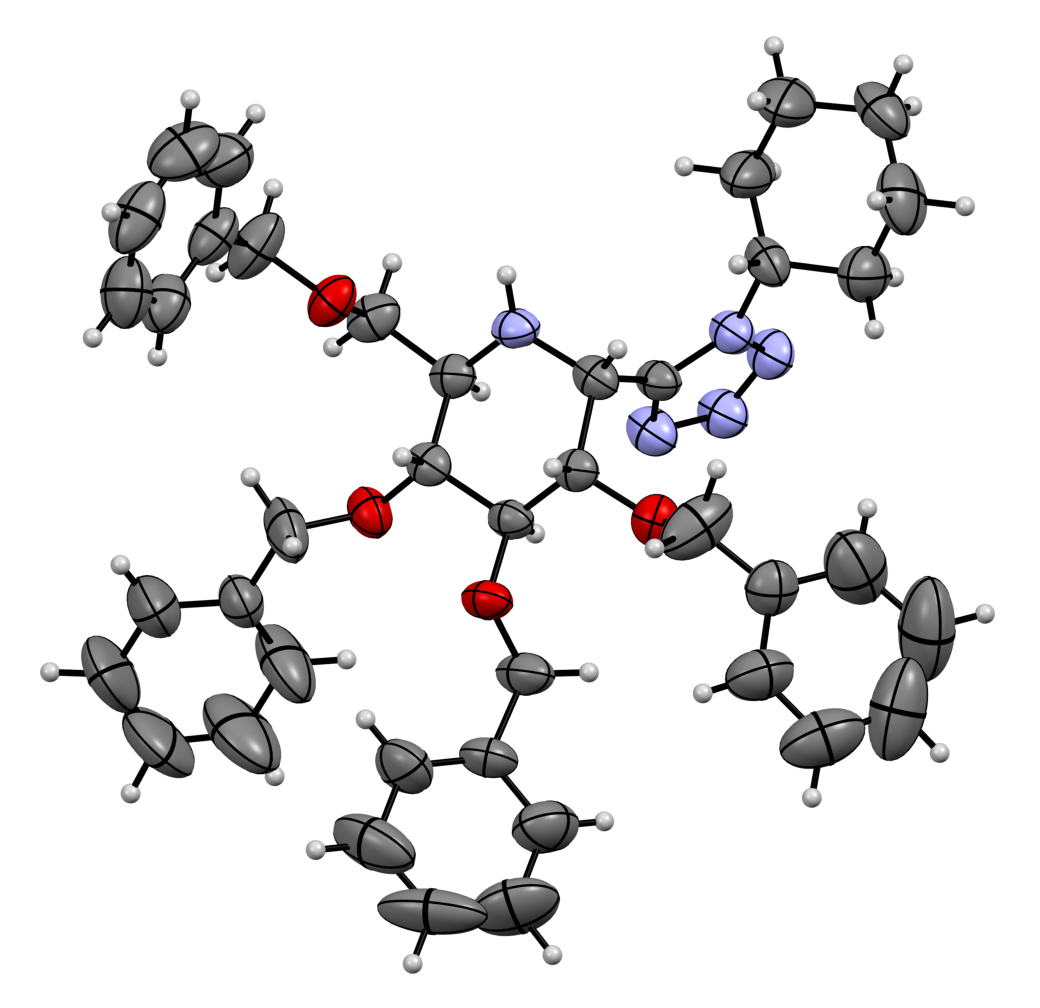
\includegraphics[height=100mm]{sugars/xray-glu-tet-cy-full.eps}
    \caption{
      Rysunek w~stylu ORTEP, przedstawiający strukturę kryształu \refcmpd{glu-tet.cy},
        w~reprezentacji elipsoid termalnych na~poziomie prawdopodobieństwa \SI{35}{\percent}.
      }
    \setfloatalignment{b}
    \label{fig:cryst-cy}
\end{figure}

\begin{table}[h]
    \begin{tabular}{l c}
        Wzór sumaryczny & \ch{C41H47N5O4} \\
        Masa molowa & \SI{673.83}{\gram\per\mol} \\
        Numer CCDC & 2001373 \\ 
        Wygląd kryształu & sześcienny, bezbarwny \\
        Układ krystalograficzny & jednoskośny \\
        Grupa przestrzenna & P $2_{1}$ \\
        a & \SI{11.7353(5)}{\angstrom} \\
        b & \SI{10.8296(4)}{\angstrom} \\
        c & \SI{15.1159(6)}{\angstrom} \\
        $\alpha$ & \SI{90}{\degree} \\
        $\beta$ & \SI{93.981(3)}{\degree} \\
        $\gamma$ & \SI{90}{\degree} \\
        Objętość & \SI{1916.42(13)}{\angstrom\cubed} \\
        Z & 2 \\
        Współczynnik R & \SI{5.77}{\percent} \\
    \end{tabular}
    \caption{
      Wybrane parametry krystalograficzne związku \refcmpd{glu-tet.cy}.
    }
    \label{tab:cryst-cy}
\end{table}

\FloatBarrier
\pagebreak
\subsection{Struktura kryształu związku \refcmpd{glu-tet.pmb}}
Kryształ odpowiedni do~pomiarów techniką rentgenografii strukturalnej otrzymałem,
  związek~\refcmpd{glu-tet.pmb} rozpuszczając w~mieszaninie heptanu i~eteru dietylowego,
  a~następnie poddając roztwór powolnemu\sidenote{Na przestrzeni kilku dni.} odparowaniu.
Poniżej prezentuję, na~\cref{fig:cryst-pmb}, strukturę przedstawioną w~stylu ORTEP
  oraz, w~\cref{tab:cryst-pmb}, wartości wybranych parametrów krystalograficznych.

\begin{figure}[h]
    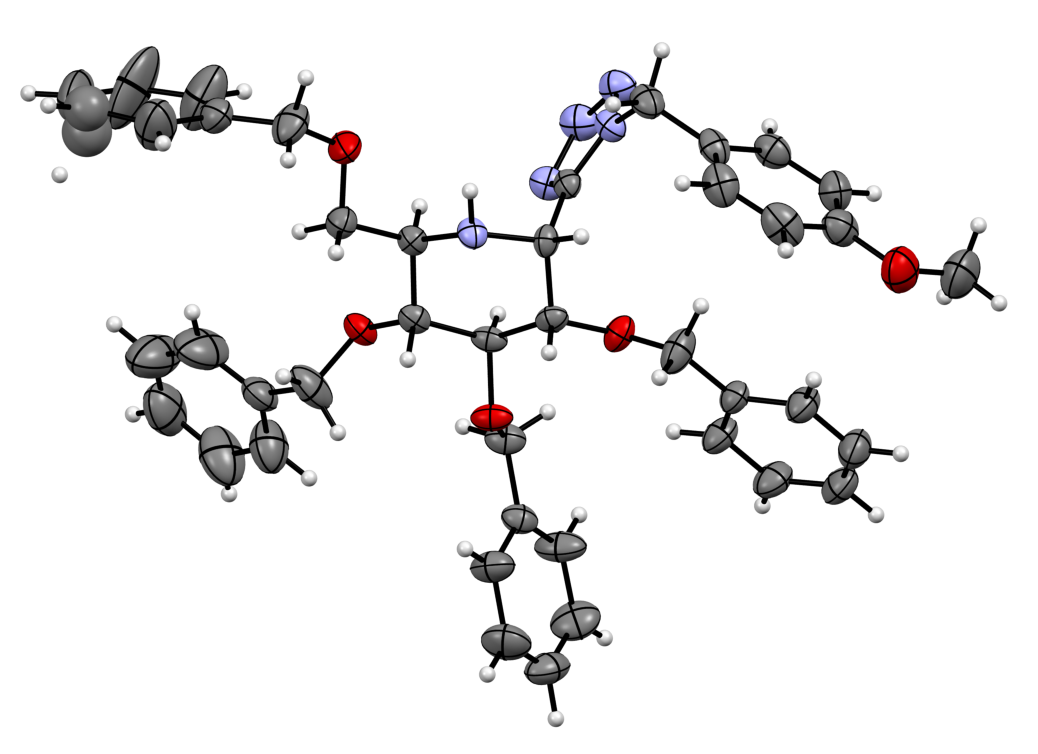
\includegraphics[height=100mm]{sugars/xray-glu-tet-pmb-full.eps}
    \caption{
      Rysunek w~stylu ORTEP, przedstawiający strukturę kryształu \refcmpd{glu-tet.pmb},
        w~reprezentacji elipsoid termalnych na~poziomie prawdopodobieństwa \SI{35}{\percent}.
      }
    \label{fig:cryst-pmb}
    \setfloatalignment{b}
\end{figure}

\begin{table}[h]
    \begin{tabular}{l c}
        Wzór sumaryczny & \ch{C43H45N5O5} \\
        Masa molowa & \SI{711.84}{\gram\per\mol} \\
        Numer CCDC & 2001372 \\ 
        Wygląd kryształu & płytkowy, żółto-bezbarwny \\
        Układ krystalograficzny & jednoskośny \\
        Grupa przestrzenna & P $2_{1}$ \\
        a & \SI{5.8938(18)}{\angstrom} \\
        b & \SI{19.634(6)}{\angstrom} \\
        c & \SI{16.520(5)}{\angstrom} \\
        $\alpha$ & \SI{90}{\degree} \\
        $\beta$ & \SI{92.037(17)}{\degree} \\
        $\gamma$ & \SI{90}{\degree} \\
        Objętość & \SI{1910.5(10)}{\angstrom\cubed} \\
        Z & 2 \\
        Współczynnik R & \SI{4.01}{\percent} \\
    \end{tabular}
    \caption{
      Wybrane parametry krystalograficzne związku \refcmpd{glu-tet.pmb}.
    }
    \label{tab:cryst-pmb}
\end{table}
\FloatBarrier

\subimport{./}{sugars-opt}